\documentclass{standalone}

\usepackage{tikz}
\usepackage{circuitikz}

\tikzset{block/.style = {draw, fill=white, very thick, rectangle, minimum height=1cm, minimum width=2cm},
         lblock/.style={draw,fill=white,very thick, rectangle, minimum height=3cm, minimum width=1cm},
         sum/.style= {draw, fill=white, very thick, circle, node distance=0.5cm}}

         
\begin{document}
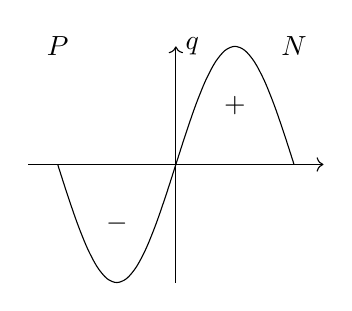
\begin{tikzpicture}[scale=1.5]
    \draw[->](-1.25,0)--(1.25,0);
    \draw[->](0,-1)--(0,1)node[right]{$q$};
    \draw[smooth, domain=-1:1]plot(\x,{sin(3.14*(\x) r)});
    \node at(0.5,0.5){$+$};
    \node at(-0.5,-0.5){$-$};
    \node at(1,1) {$N$};
    \node at(-1,1){$P$};
\end{tikzpicture}
\end{document}